\documentclass{article}
\usepackage{fullpage}
\usepackage{hyperref}
\usepackage{authblk}
\usepackage[utf8]{inputenc}

\title{Using vulcan, a package that combines regulatory networks and ChIP-Seq data to identify chromatin-binding cofactors}
\author[1]{Federico M. Giorgi}
\author[1]{Andrew N. Holding}
\author[1]{Florian Markowetz}
\affil[1]{Cancer Research UK, Cambridge Institute, Robinson Way, Cambridge United Kingdom}
\date{\today}

\usepackage{Sweave}
\begin{document}
\Sconcordance{concordance:vulcan.tex:vulcan.Rnw:%
1 13 1 1 0 16 1 1 4 1 2 1 0 2 1 3 0 1 2 3 1 1 2 4 0 2 2 4 0 1 2 5 1 1 3 %
2 0 1 1 3 0 1 2 1 1 1 3 2 0 1 1 3 0 1 2 1 1 1 3 5 0 1 2 1 1 1 3 2 0 1 2 %
4 0 1 2 2 1 1 2 4 0 1 2 3 1 1 2 1 0 1 1 4 0 1 2 6 1 1 2 1 0 3 1 3 0 2 2 %
5 0 1 2 2 1 1 2 1 0 5 1 3 0 1 2 3 1 1 2 1 0 1 2 1 0 4 1 1 3 1 0 4 1 4 0 %
1 2 11 1}

\maketitle

%-----------
\section{Overview of VULCAN}\label{sec:overview}
Vulcan (VirtUaL ChIP-Seq Analysis through Networks) is a pipeline that combines ChIP-Seq data and regulatory networks to obtain transcription factors that are likely affected by a specific stimulus. In order to do so, our package combines strategies from different BioConductor packages: \emph{DESeq} for data normalization, \emph{ChIPpeakAnno} and \emph{DiffBind} for annotation and definition of ChIP-Seq genomic peaks, \emph{csaw} to define optimal peak width and \emph{viper} for applying a regulatory network over a differential binding signature.
Usage of gene regulatory networks to analyze biological systems has witnessed an exponential increase in the last decade, due to the ease of obtaining genome-wide expression data (Margolin et al., 2005; Giorgi et al., 2013; Castro et al., 2015). Recently, the VIPER approach to interrogate these network models has been proposed to infer transcription factor activity using the expression of a collection of their putative targets, i.e. their regulon (Alvarez et al., 2016). In the VIPER algorithm, gene-level differential expression signatures are obtained for either individual samples (relative to the mean of the dataset) or between groups of samples, and regulons are tested for enrichment. Ideally, TF regulons can be tested on promoter-level differential binding signatures generated from ChIP-Seq experiments, in order to ascertain the global change in promoter occupancy for gene sets. In our study, we propose an extension of the VIPER algorithm to specifically analyze TF occupancy in ChIP-Seq experiments. Our VULCAN algorithm uses ChIP-Seq data obtained for a given TF to provide candidate coregulators of the response to a given stimulus. The analysis is based on identifying differentially bound genes and testing their enrichment in the regulon of potential co-regulatory factors.

%--------
\section{Citation}
Giorgi FM, Holding AN \& Markowetz F. Network Dynamics of early ER-alpha promoter binding in response to estradiol. Genome Biology (Submitted).
%--------
\section{Installation of \emph{vulcan} package}
VULCAN requires the R-system (\url{http://www.r-project.org}), and the \emph{vulcandata} package to run the examples.
After installing R, all required components can be obtained with:


\begin{Schunk}
\begin{Sinput}
> source("http://bioconductor.org/biocLite.R")
> biocLite("vulcandata")
> biocLite("vulcan")
\end{Sinput}
\end{Schunk}

%----
\section{Getting started}
As first step, we have to load the vulcan package with:
\begin{Schunk}
\begin{Sinput}
> library(vulcan)
\end{Sinput}
\end{Schunk}
Only to run the examples, a set of reduced BAM files can be accessed by loading the \emph{vulcandata} package:
\begin{Schunk}
\begin{Sinput}
> library(vulcandata)
\end{Sinput}
\end{Schunk}


%-------
\section{Running an example VULCAN pipeline}

\subsection{Generate a example annotation file}
\begin{Schunk}
\begin{Sinput}
> # Generate an annotation file from the dummy ChIP-Seq dataset
> vfile<-"deleteme.csv"
> vulcansheet(vfile)
\end{Sinput}
\end{Schunk}

\subsection{Import ChIP-Seq information}
\begin{Schunk}
\begin{Sinput}
> # Import BAM and BED information into a list object
> vobj<-vulcan.import(vfile)
> unlink(vfile)
\end{Sinput}
\end{Schunk}

\subsection{Annotate peaks}
\begin{Schunk}
\begin{Sinput}
> # Annotate peaks to gene names
> vobj<-vulcan.annotate(vobj,lborder=-10000,rborder=10000,method="sum")
\end{Sinput}
\end{Schunk}

\subsection{Peak abundance normalization}
\begin{Schunk}
\begin{Sinput}
> # Normalize data for VULCAN analysis
> vobj<-vulcan.normalize(vobj)
> # Detect which conditions are present in our imported object
> names(vobj$samples)
\end{Sinput}
\end{Schunk}

\subsection{Load an ARACNe network}
We will use a regulon object as specified in the \emph{viper} package, named "network"
\begin{Schunk}
\begin{Sinput}
> load(system.file("extdata","network.rda",package="vulcan",mustWork=TRUE))
\end{Sinput}
\end{Schunk}

\subsection{Run VULCAN}
Once we have prepared 1) the ChIP-Seq annotated and normalized object and 2) a gene regulatory network, we can run the VULCAN pipeline.
We can reduce the minimum regulon size, since in the \emph{vulcandata} example only one chromosome was used, and the networks would otherwise have too few hits. We can then visualize the output using the msviper plotting function
\begin{Schunk}
\begin{Sinput}
> vobj_analysis<-vulcan(vobj,network=network,contrast=c("t90","t0"),minsize=5)
> plot(vobj_analysis$msviper,mrs=7)
\end{Sinput}
\end{Schunk}
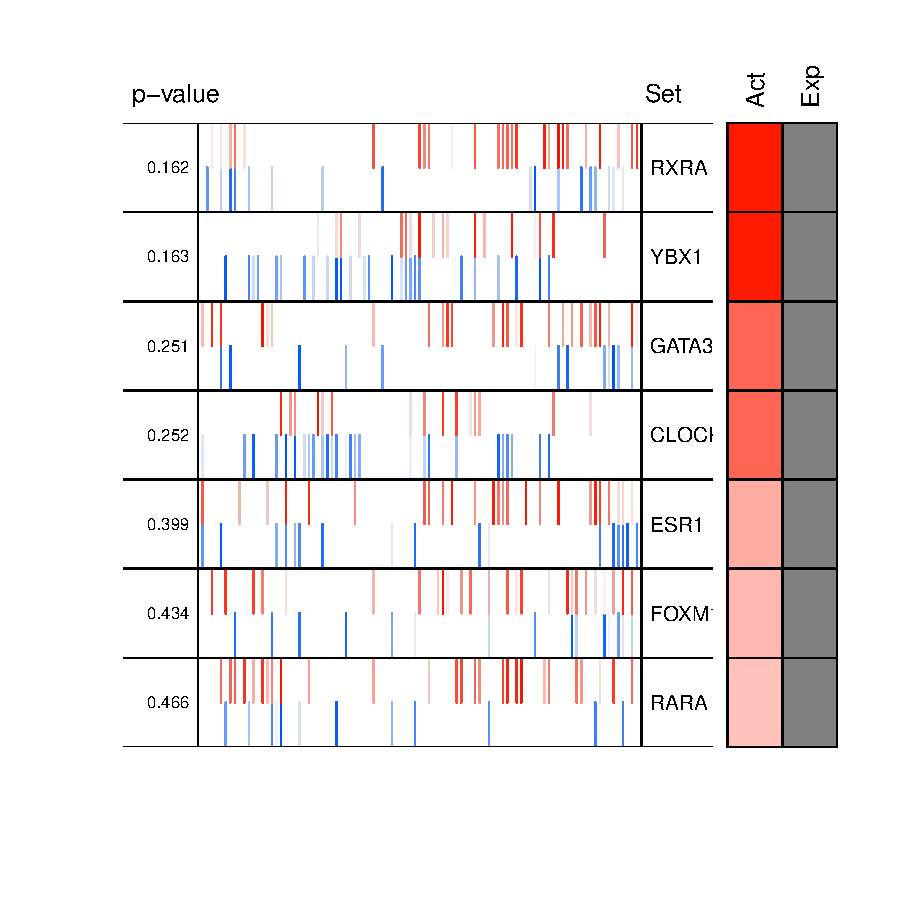
\includegraphics{vulcan-010}


%-------
\section{More convenience tools for ChIP-Seq functional data analysis}

\subsection{Gene Set Enrichment Analysis}
VULCAN contains a GSEA (Subramanian et al., 2005) implementation that can fit a Pareto tail distribution for p-value estimation. In the following example, we generate an artificial signature of 1000 genes with normally-distributed positive expression. The gene set that is evaluated is composed by 50 genes randomly picked from one of the tails
\begin{Schunk}
\begin{Sinput}
> reflist<-setNames(-sort(rnorm(1000)),paste0("gene",1:1000))
> set<-paste0("gene",sample(1:200,50))
> obj<-gsea(reflist,set,method="pareto")
> obj$p.value
\end{Sinput}
\end{Schunk}
The GSEA object can be plotted
\begin{Schunk}
\begin{Sinput}
> plot_gsea(obj)
\end{Sinput}
\end{Schunk}
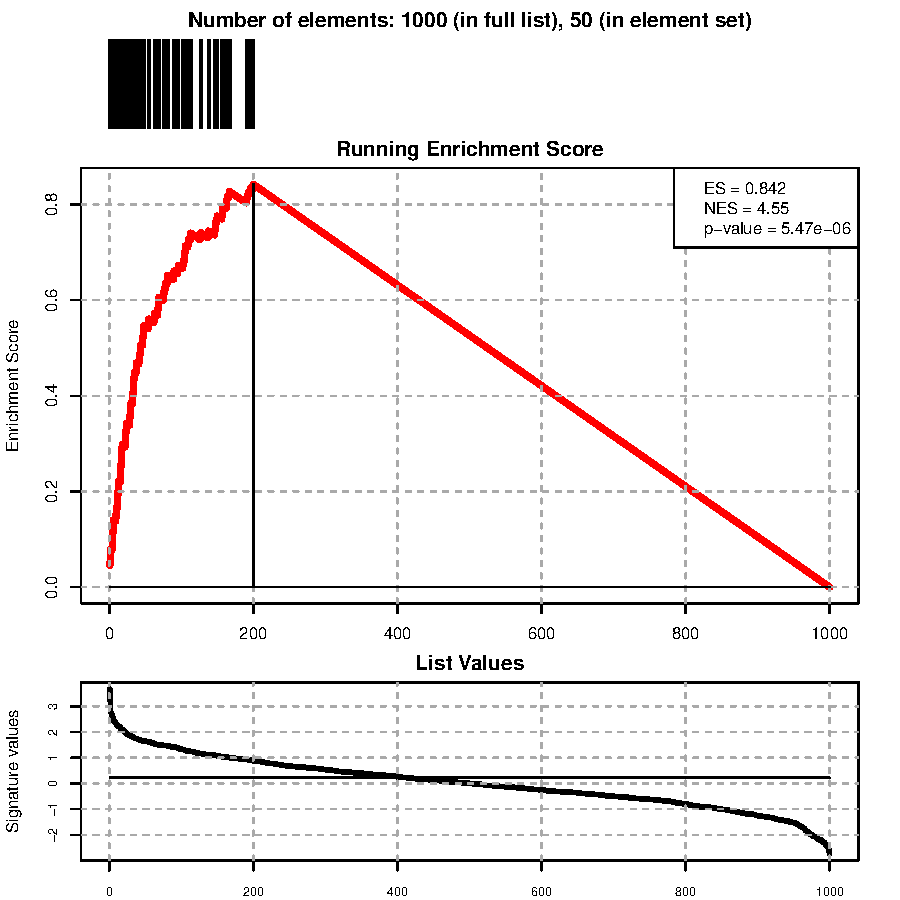
\includegraphics{vulcan-012}

\subsection{Rank Enrichment Analysis}
Rank Enrichment Analysis (REA Calculates) enrichment of groups of objects over a vector of values associated to a population of objects using a linear algebraic matrix multiplication.
\begin{Schunk}
\begin{Sinput}
> signatures<-setNames(-sort(rnorm(1000)),paste0("gene",1:1000))
> set1<-paste0("gene",sample(1:200,50))
> set2<-paste0("gene",sample(1:1000,50))
> groups<-list(set1=set1,set2=set2)
> obj<-rea(signatures=signatures,groups=groups)
> obj
\end{Sinput}
\end{Schunk}


\subsection{Convenience functions}
The function \emph{kmgformat} will convert thousand numbers to K, millions to M, billions to G, trillions to T, quadrillions to P. The function \emph{val2col} converts a distribution of numbers to a distribution of colors.
\begin{Schunk}
\begin{Sinput}
> par(mfrow=c(1,2))
> # Thousands
> set.seed(1)
> a<-runif(1000,0,1e4)
> plot(a,yaxt="n")
> kmg<-kmgformat(pretty(a))
> axis(2,at=pretty(a),labels=kmg)
> # Millions to Billions
> set.seed(1)
> a<-runif(1000,0,1e9)
> plot(a,yaxt="n",pch=20,col=val2col(a))
> kmg<-kmgformat(pretty(a))
> axis(2,at=pretty(a),labels=kmg)
\end{Sinput}
\end{Schunk}
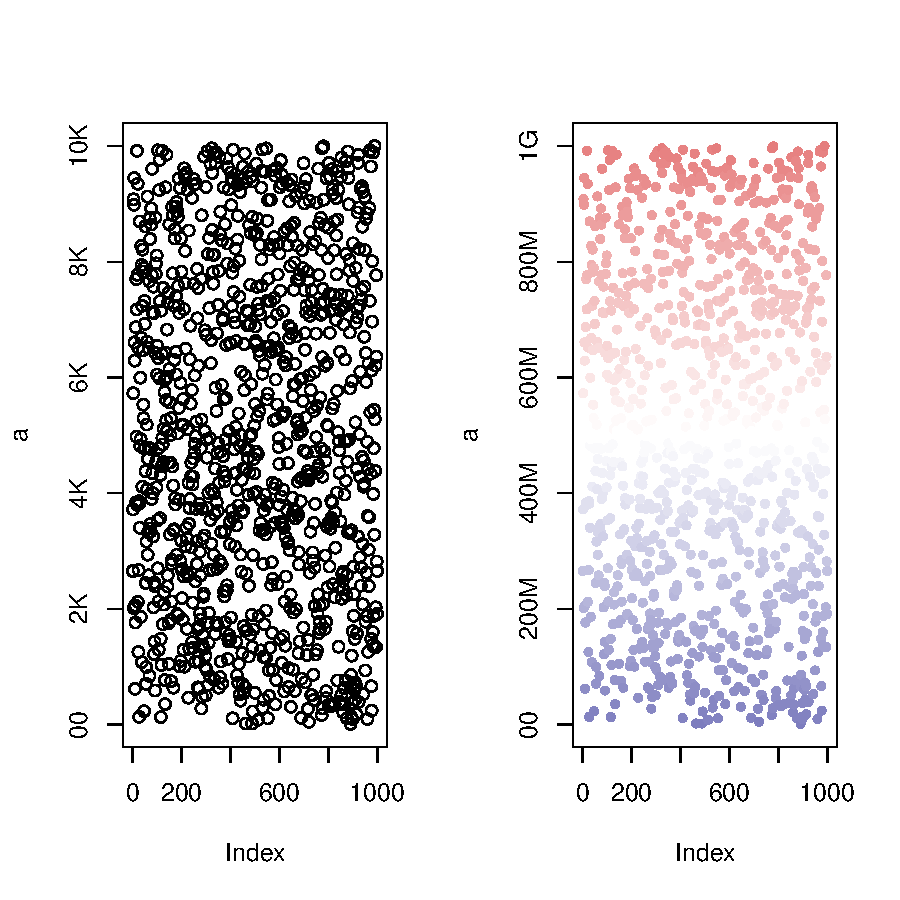
\includegraphics{vulcan-014}


%-----------
\begin{thebibliography}{99}
\bibitem{Alvarez2013} Alvarez, M.J., Shen, Y., Giorgi, F.M., Lachmann, A., Ding, B.B., Ye, B.H., \& Califano, A. (2016). Functional characterization of somatic mutations in cancer using network-based inference of protein activity. Nature Genetics.
\bibitem{Margolin2005} Margolin, A.A., Nemenman, I., Basso, K., Wiggins, C., Stolovitzky, G., Dalla Favera, R., \& Califano, A. (2006). ARACNE: an algorithm for the reconstruction of gene regulatory networks in a mammalian cellular context. BMC bioinformatics, 7(1), S7.
\bibitem{Castro2015} Castro, M.A., de Santiago, I., Campbell, T.M., Vaughn, C., Hickey, T.E., Ross, E., Tilley, W.D., Markowetz, F., Ponder, B.A. \& Meyer, K.B., 2015. Regulators of genetic risk of breast cancer identified by integrative network analysis. Nature genetics.
\bibitem{Giorgi2013} Giorgi, F.M., Del Fabbro, C., \& Licausi, F. (2013). Comparative study of RNA-seq-and microarray-derived coexpression networks in Arabidopsis thaliana. Bioinformatics, 29(6), 717-724.
\bibitem{Subramanian2005} Subramanian, A., Tamayo, P., Mootha, V.K., Mukherjee, S., Ebert, B.L., Gillette, M.A. \& Mesirov, J.P. (2005). Gene set enrichment analysis: a knowledge-based approach for interpreting genome-wide expression profiles. Proceedings of the National Academy of Sciences, 102(43), 15545-15550.
\end{thebibliography}
%----------
\end{document}
